\documentclass[11pt, oneside]{article}   	% use "amsart" instead of "article" for AMSLaTeX format
\usepackage[margin=1in]{geometry}                		% See geometry.pdf to learn the layout options. There are lots.
\geometry{letterpaper}                   		% ... or a4paper or a5paper or ... 
%\geometry{landscape}                		% Activate for rotated page geometry
%\usepackage[parfill]{parskip}    		% Activate to begin paragraphs with an empty line rather than an indent
\usepackage{graphicx}				% Use pdf, png, jpg, or eps§ with pdflatex; use eps in DVI mode
								% TeX will automatically convert eps --> pdf in pdflatex		
\usepackage{amssymb}
%usepackage{undertilde}
\usepackage[numbered,framed]{matlab-prettifier}

\usepackage[T1]{fontenc}
\usepackage{mathtools}  % loads »amsmath«
\usepackage{physics}
\usepackage{listings}

\usepackage{float}
\restylefloat*{figure}

\setlength{\parskip}{0.5em}

%SetFonts
\newcommand\Rey{\mbox{\textit{Re}}}

\title{\vspace{-6ex} Assignment 3- Parallel Computation of Pi \\ {CSCI 596: Scientific Computing \& Visualization}  \vspace{-2ex}}
\author{Anup V Kanale}
\date{\vspace{-2ex}\today}							% Activate to display a given date or no date

\begin{document}
\maketitle \vspace{-5ex}

This purpose of this assignment is to understand the meaning of scalability analysis for parallel programs using a simple example-- parallel computation of $\pi$.

\vspace{-2ex} \section{MPI program to compute $\pi$}
\begin{figure}[!htbp]
	\centering
	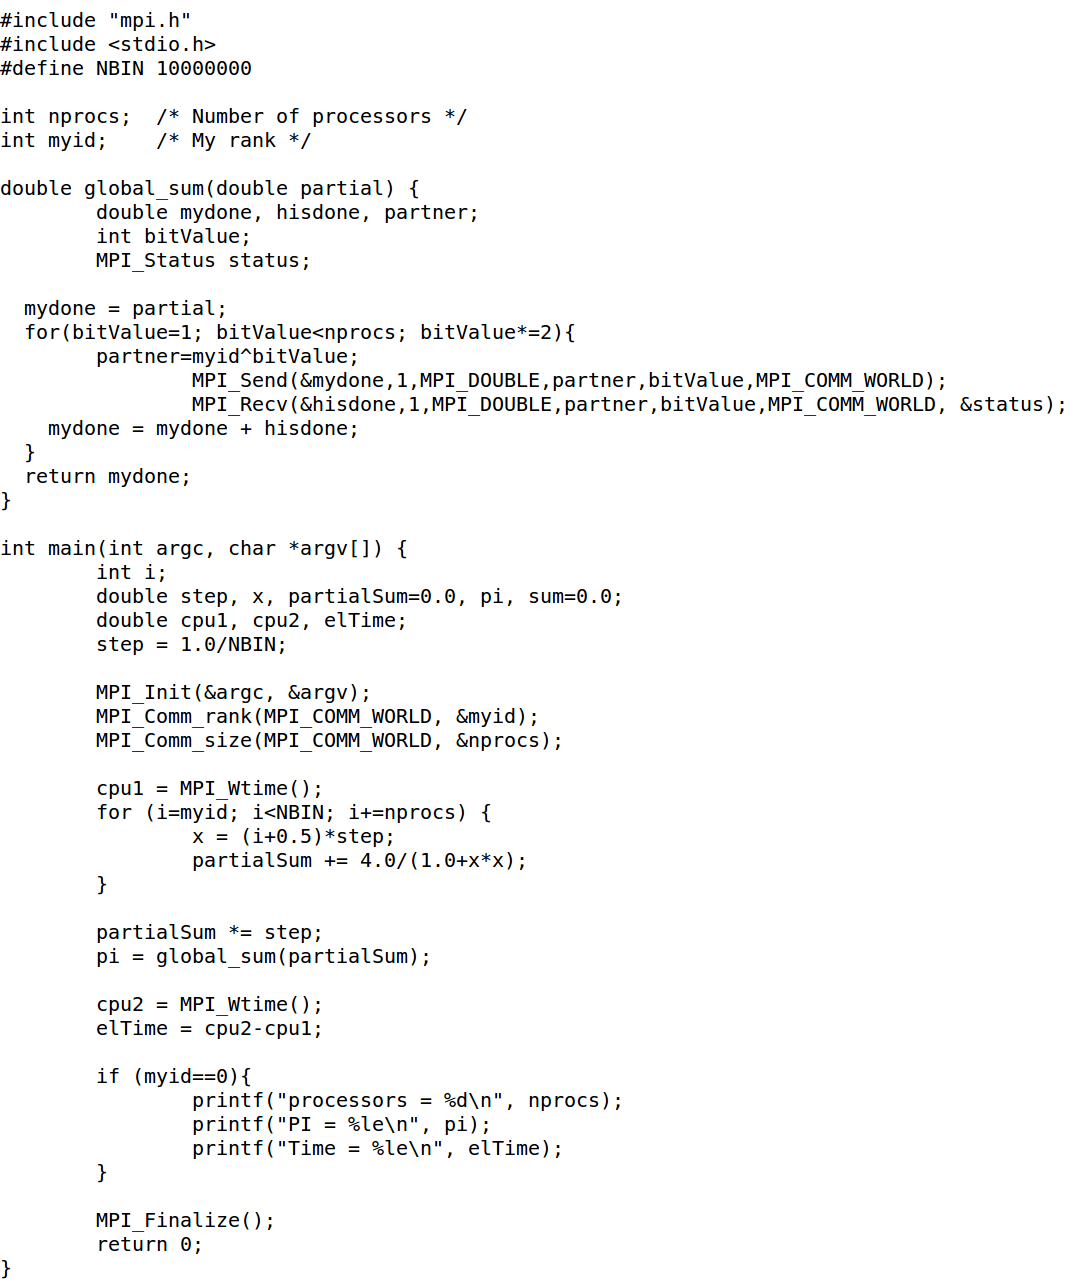
\includegraphics[scale=0.2]{C-code.png}
	\caption{C-program to compute pi parallely}
\end{figure}

\vspace{-2ex} \section{Scalability}
In this section, the relationship between the number of processors being used, and the size of the problem is explored. Before we delve into it, I will discuss a little about using the hpc cluster at USC in interactive mode.

\subsection{Interactive job at HPC}
First log into the hpc account as usual using ssh protocol. The difference between submitting a normal job using a pbs file and interactive mode is that in the latter 
To run an interactive job \texttt{qsub -I -l walltime=01:00:00 -l nodes=2:ppn=4}

Let us now quantify the scalability of \texttt{global.pi.c}. There are two metrics here-- fixed-problem size scaling and the isogranular scaling.

\subsection{Fixed problem-size scaling}
In this case, we keep the size of the problem constant, i.e., we run the program \texttt{global\_pi.c} for a fixed number of quadrature points, \texttt{NBIN} $= 10^7$, for different number of compute nodes (or processors). The below plots summarizes the results.
\begin{figure}[!htbp]
	\centering
	\begin{minipage}{0.45\textwidth}
		\centering
		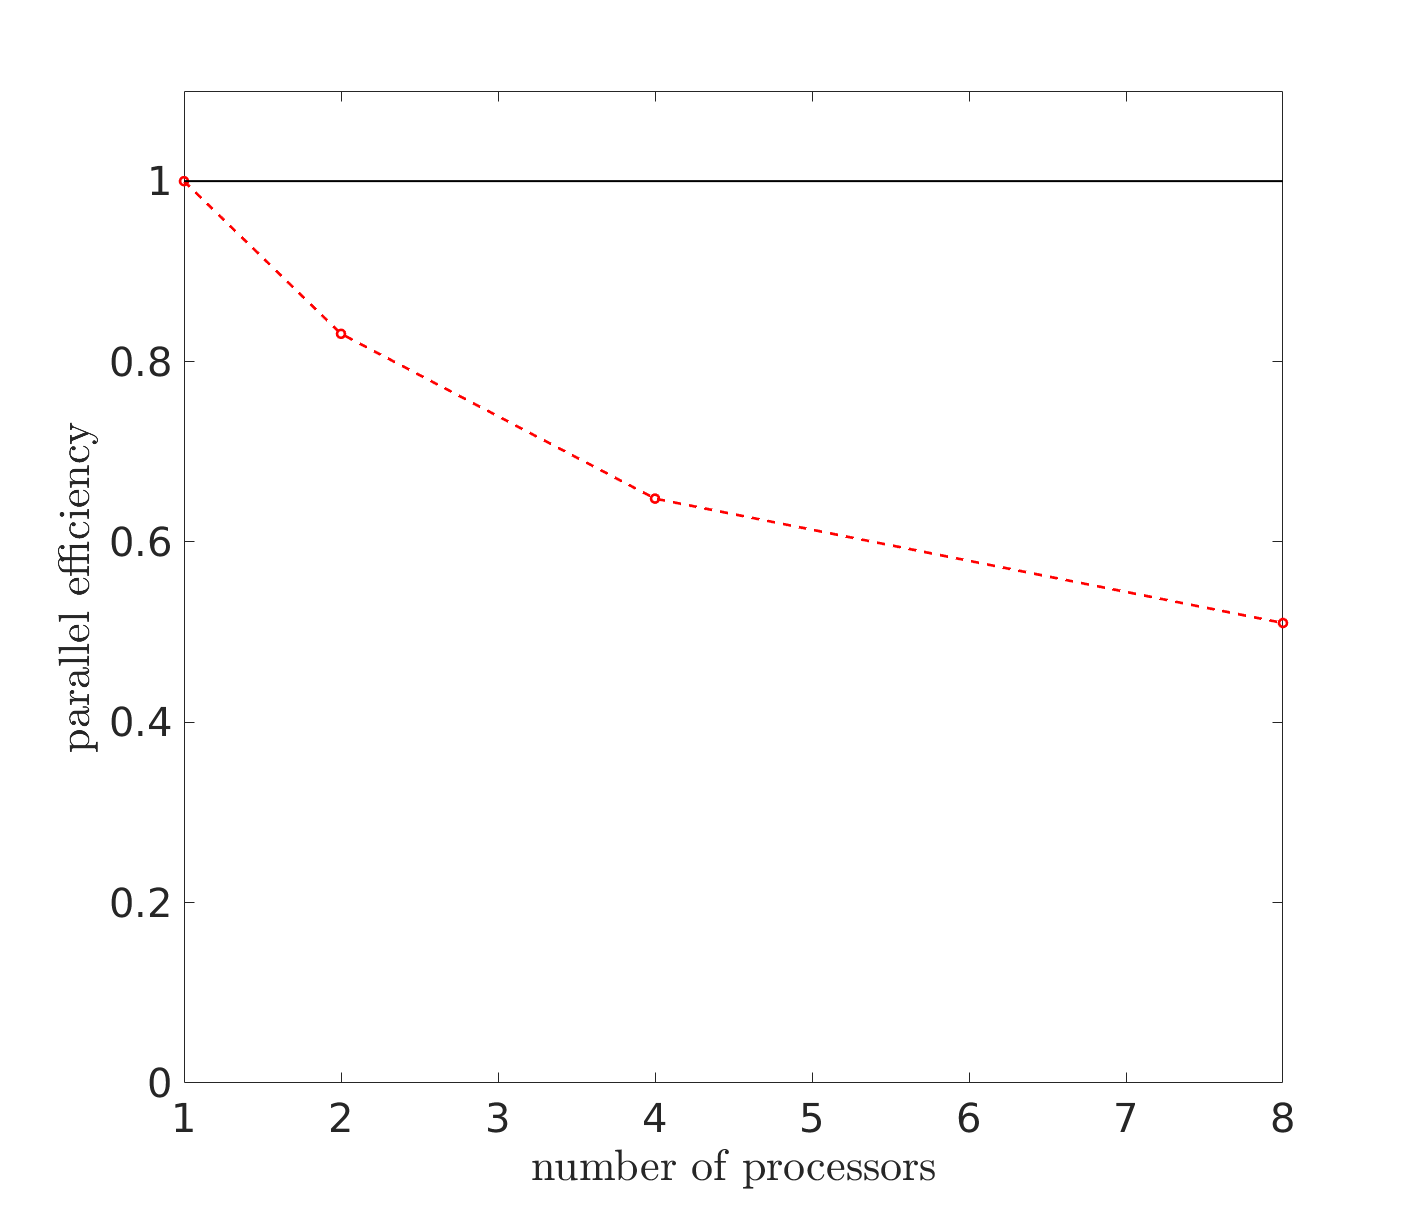
\includegraphics[width=1.2\textwidth]{fixed_probsize_Eff.png} % first figure itself
		\caption{Fixed problem-size parallel efficiency}
	\end{minipage}\hfill
	\begin{minipage}{0.48\textwidth}
		\centering
		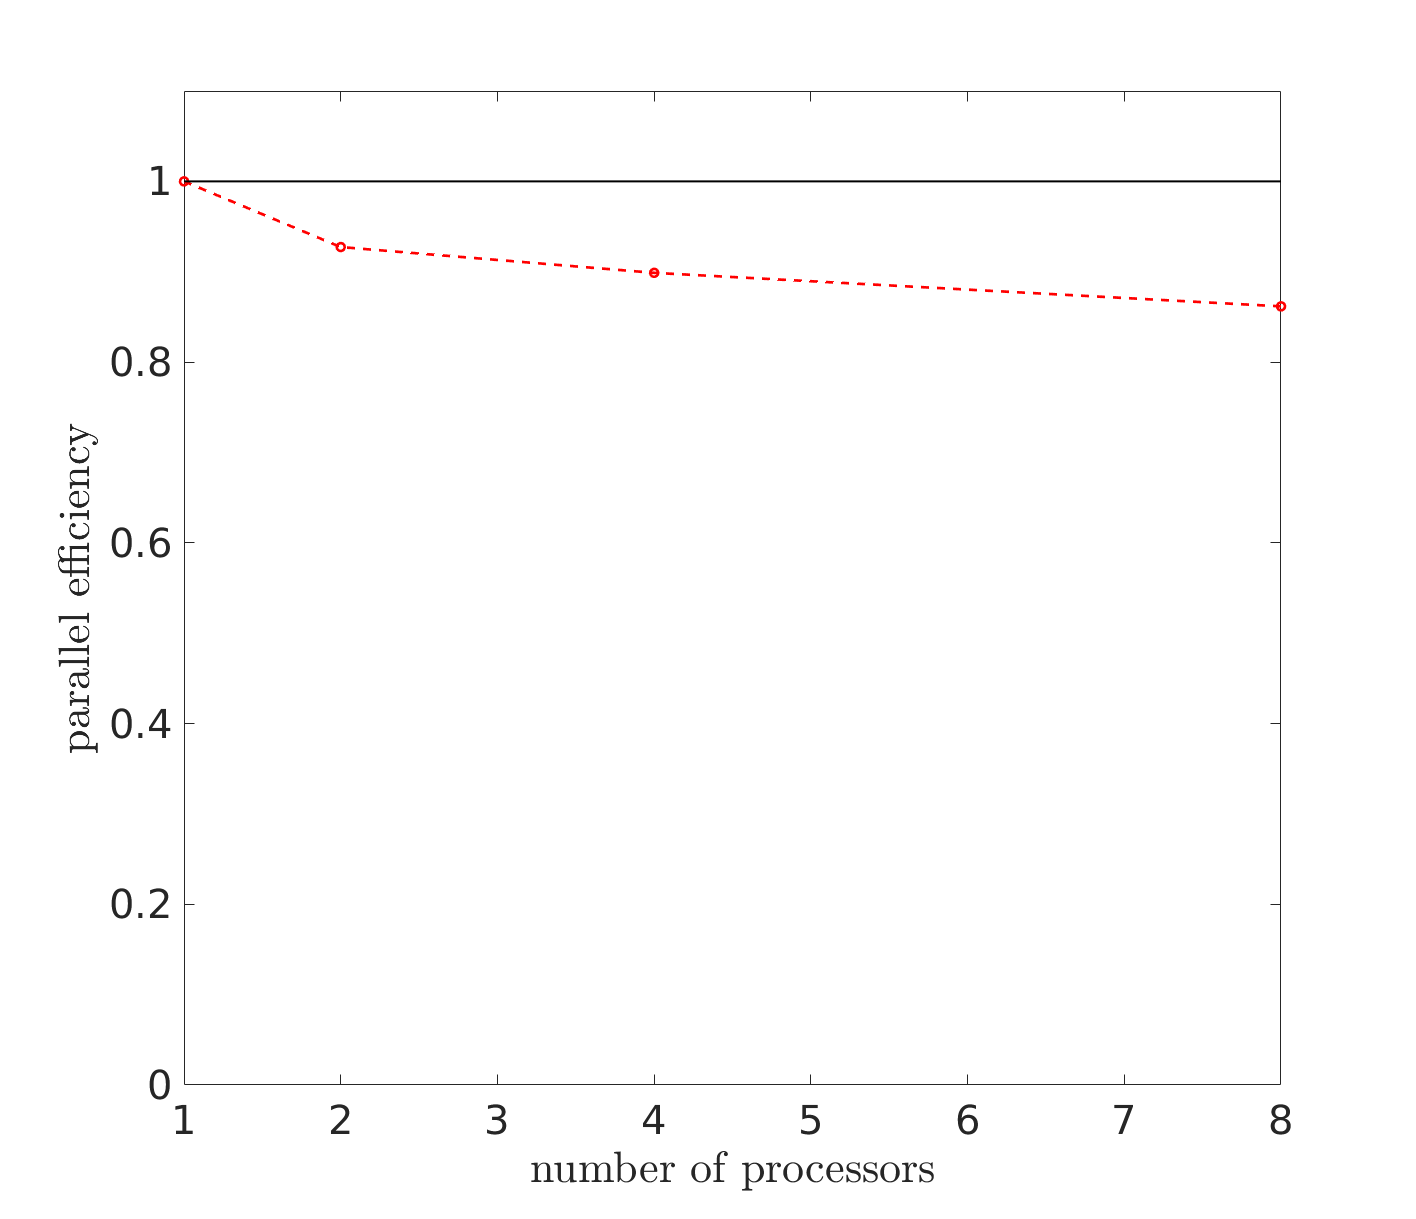
\includegraphics[width=1.2\textwidth]{isogranular_Eff.png} % second figure itself
		\caption{Isogranular parallel efficiency}
	\end{minipage}
\end{figure}

\subsection{Fixed problem-size scaling}
In this case, the size of the problem scales with the number of processors, i.e., we run the program \texttt{global\_pi.c} for a \texttt{NBIN} $= 10^7$. \textit{per processor}. So for 1 processor, \texttt{NBIN} $= 10^7$, for 2 processors, \texttt{NBIN} $= 2 \times10^7$, and for $P$ processors,  \texttt{NBIN} $= P \times10^7$. The below plot summarises the results.

\vspace{-2ex} \section{Conclusions}
As seen from the above results, parallel computation can get very inefficient as the number of processors are increased for the same problem size. This is because more time is lost in communication between processors than for the actual computation. However, isogranular parallel efficiency decays at a much slower rate.
\vspace{-2ex} \section{Potential Issues}
\begin{enumerate}
	\item Run time variance
	\begin{itemize}
		\item Heterogeneous cluster--> run all P in one PBS file
		\item Shared network--> run multiple times and take min
	\end{itemize}
	\item Effficiency>1
	\begin{itemize}
	\item Measurement noise
	\item Cache effect (only fixed problem size). won't happened for this HW.
	\end{itemize}
\end{enumerate}

\end{document}